\section{Entity relationship diagram}
\subsection{Introduction}
\begin{flushleft}
Dans cette partie, je vais vous expliquer les ajouts apportés à la base de données de la base du projet. 
\end{flushleft}
\begin{flushleft}
De ce fait, il me semblait plus judicieux de garder dans ce rapport que les sections jouant un rôle primordial dans la base de données pour l'extension.
\end{flushleft}
\begin{flushleft}
Vous pourrez donc y retrouver le fonctionnement de certains attributs ainsi que les clés primaires et étrangères.
\end{flushleft}
\begin{flushleft}
Comme vous le remarquerez, le choix de séparer "portefeuilles" de "portefeuilles invités" joue encore un rôle important dans la manière de réaliser ce diagramme.
\end{flushleft}

\subsection{Utilisateur}
\begin{flushleft}
De la même manière que pour la base du projet, partons du principe qu'un fournisseur, un client et un client "propriétaire" (gestionnaire) sont des utilisateurs de l'application.\newline
De ce fait, utilisons donc l'identifiant "id".
\end{flushleft}

\begin{flushleft}
On aura donc :
\end{flushleft}

\begin{enumerate}
\item PK(utilisateur) = id
\item FK(utilisateur) REFS fournisseur = id
\item FK(utilisateur) REFS client = id
\item FK(utilisateur) REFS client\_propriétaire = id
\end{enumerate}

\newpage
\subsection{Portefeuille invité}
\begin{flushleft}
Vous remarquerez que ce qui le différencie principalement du "portefeuille" sont les attributs suivants:
\end{flushleft}
\begin{enumerate}
\item \textbf{les permissions }: \newline
Les permissions sont donc celles attribuées à un client (invité), c'est à dire, "lecture" ou "lecture et écriture". \newline
Ce qui explique donc la présence du binary(1) représentant les deux possibilités.

\item \textbf{l'id du propriétaire} :\newline
Son ajout est lié au fait qu'il s'agit d'un élément non négligeable. \newline 
Le but étant de le récupérer pour obtenir la totalité des informations essentielles.\newline
En outre, son id est différent de l'id client.
\end{enumerate}

\begin{flushleft}
Il est important de noter que l'id client dans ce cas est en fait le client invité ayant la possibilité de lire ou de lire et écrire dans les portefeuilles invités et étant donc gestionnaire dans la partie portefeuille.
\end{flushleft}

\begin{flushleft}
On a donc en terme de clés :
\end{flushleft}

\begin{enumerate}
\item PK(portefeuille) = adresse et id\_client :\newline
La table va stocker toutes les invitations de tous les portefeuilles et il y aura donc plusieurs invités pour une adresse.
\item FK(portefeuille) REFS client = id\_client
\item FK(portefeuille) REFS client\_propriétaire = id\_propriétaire
\end{enumerate}

\subsection{Contrat du portefeuille}
\begin{flushleft}
Cette section ne sera pas affectée, la seule différence avec la base réside dans le fait que cette dernière est également liée aux portefeuilles invités.
\end{flushleft}
\begin{flushleft}
En effet, tout comme les "portefeuilles", les "portefeuilles invités" doivent être aussi liés aux contrats.
\end{flushleft}

\newpage
\subsection{Diagramme}
\begin{figure}[h]
\centering
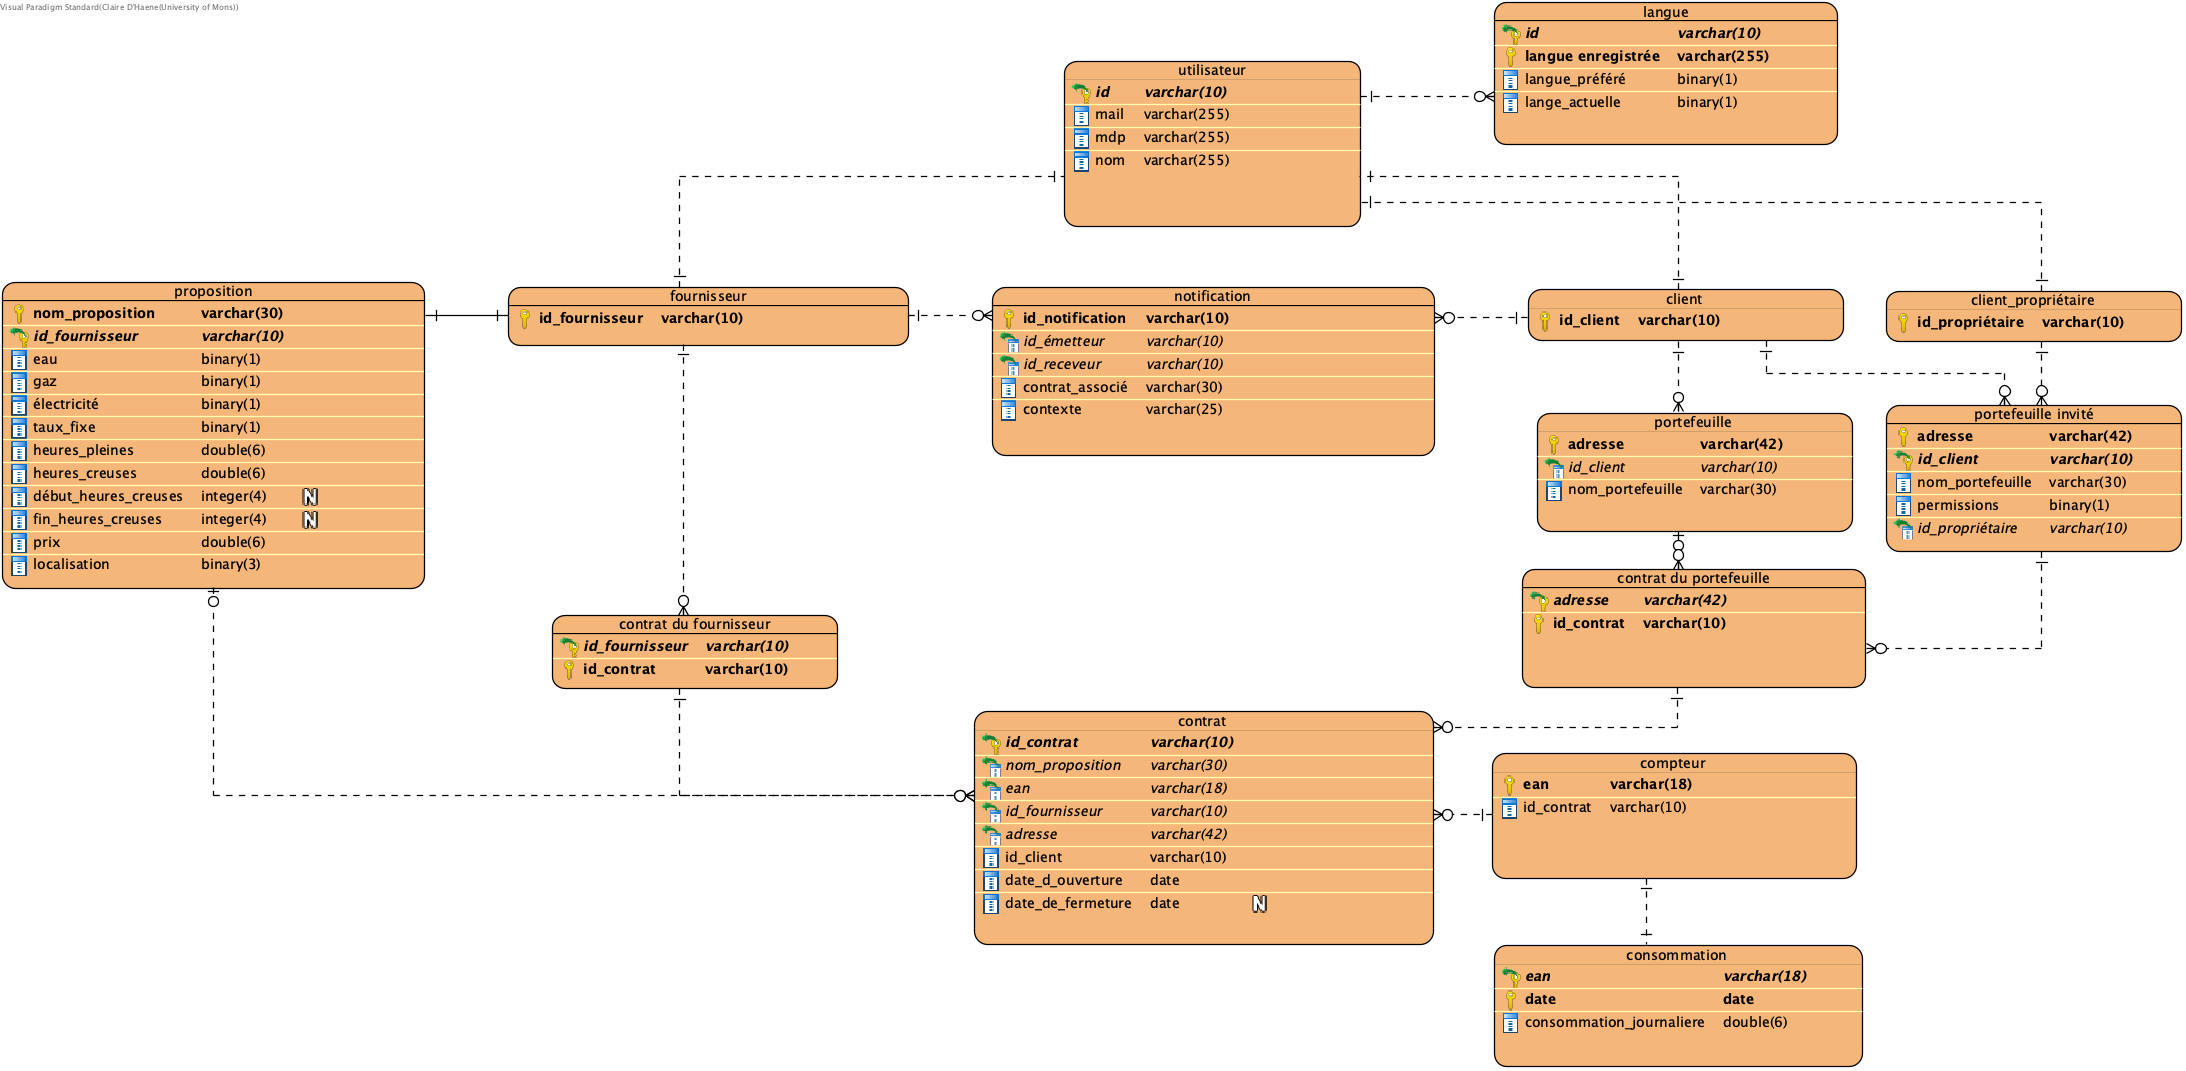
\includegraphics[width = 1\textwidth]{Extension-claire/BDD-claire/img/BDD-claire.png}
\end{figure}